% Template for ISBI-2018 paper; to be used with:
%          spconf.sty  - ICASSP/ICIP LaTeX style file, and
%          IEEEbib.bst - IEEE bibliography style file.
% --------------------------------------------------------------------------
\documentclass{article}
\usepackage{spconf,amsmath,amsfonts,amssymb,graphicx,cite}

% Example definitions.
% --------------------
\def\x{{\mathbf x}}
\def\L{{\cal L}}
\DeclareMathOperator*{\argmax}{arg\,max}

% Title.
% ------
\title{3D Neuron Pose Estimation from Calcium Image Stack Sequences Using Neuron Plane Model}
%
% Single address.
% ---------------
\name{S. Gulyanon$^1$, W. D. Tracy$^2$, L. He$^2$, and G. Tsechpenakis$^3$ \thanks{This work is supported by NSF/DBI [$\#$1252597]: `CAREER: Modeling the structure and dynamics of neuronal circuits in the \emph{Drosophila} larvae using image analytics' awarded to G. Tsechpenakis.} \vspace{-5pt}}
\address{\small{$^1$Department of Computer Science, Thammasat University, Thailand;}\\
	\small{$^2$ Department of Biology, Indiana University, USA;} \\
	\small{$^3$Computer and Information Science Department, Indiana University-Purdue University Indianapolis, USA;} \vspace{-2pt} \\}
%
%
% For example:
% ------------
%\address{School\\
%	Department\\
%	Address}
%
% Two addresses (uncomment and modify for two-address case).
% ----------------------------------------------------------
%\twoauthors
%  {A. Author-one, B. Author-two\sthanks{Thanks to XYZ agency for funding.}}
%	{School A-B\\
%	Department A-B\\
%	Address A-B}
%  {C. Author-three, D. Author-four\sthanks{The fourth author performed the work
%	while at ...}}
%	{School C-D\\
%	Department C-D\\
%	Address C-D}
%
% More than two addresses
% -----------------------
% \name{Author Name$^{\star \dagger}$ \qquad Author Name$^{\star}$ \qquad Author Name$^{\dagger}$}
%
% \address{$^{\star}$ Affiliation Number One \\
%     $^{\dagger}$}Affiliation Number Two
%
\begin{document}
%\ninept
%
\maketitle
%
\begin{abstract}
It is known that the sensory neurons control the locomotion but we do not know how this happens. The lack of robust tools for simultaneous quantification of both morphology and neuronal activity in calcium images hinders the progress. The main issues are that these calcium volumes are noisy, have low resolution in Z-axis, contain significant deformations during movement, and suffer from the characteristics of calcium images. In this work, we developed the interactive tracking method of surfaces enclosing neurons. Tracking neurons indirectly helps handle these issues, and improve the efficiency and robustness for 3D pose estimation, while little user intervention is required to aid with dendrite detection. Our method finds the best fitting surface using our neuron plane model by incorporating the image appearance, local shape, as well as domain knowledge about neuron morphology and locomotion. We validated our results using time-lapse calcium image stacks of larval Drosophila sensory neuron.
\end{abstract}
%
\begin{keywords}
Interactive pose estimation, pictorial structures, calcium images, neuron morphology
\end{keywords}
%
\section{Introduction}
\label{sec:intro}
% why we want to study the link between locomotion and neuron activity
Over decades, we know that sensory neurons control the locomotion process but we poorly understand the molecular mechanisms that determine the responses of the proprioceptive cells. Although we aware that the absence of sensory signals from these proprioceptors causes the uncoordinated and slow locomotion is uncoordinated, it is unknown exactly what these signals are \cite{Hughes2007}. To answer this question, we use high speed confocal microscopy to describe how the dendrites of proprioceptive neurons in larval Drosophila are deformed by the forces of crawling motions. This is possible because these sensory neurons lie beneath the epidermis of larval Drosophila \cite{Grueber2002}. Surprisingly, the pattern of deformation for a given neuron is unique in each direction of motion \cite{Gulyanon2018a}; and two particular neurons (dda-D and dda-E) show strong activation level during the locomotion. To gain insight into the underlying mechanisms, we must expose the link between the change in morphology and the neuronal activity of the neuron pair.

% why do we need to analyze the calcium images
Fortunately, calcium imaging holds the key to understanding the relationship between neuron morphology and neuronal activity because its intensity is proportional to the neuronal firing level; as a result calcium images also show the location of active regions in neurons. Hence, the time-lapse calcium imagery allows us to observe both neuron morphology and neuronal activity simultaneously. Due to the large amount of image sequences required for learning the link between locomotion and sensory neuron activity, the manual approach is infeasible; and the lack of robust tools for simultaneous quantification of both morphology and neuron activity hinders the progress.

% challenge
The quantification of neuronal morphology in calcium images is challenging due to four factors. First, it involves tracking neurons in 3D over noisy calcium image sequences. Second, time-lapse image stacks have low resolution in Z-axis due to the limitation of imaging system. Third, the deformation of neurons during the locomotion can be severe and creates blurry images and large displacement. Last, the most challenging problem is the characteristics of calcium images, which has low intensity when neurons are inactive so the neurons are barely visible in such cases. Neurons have high intensity when they are active but they are usually deforming in those frames as well (fig.~\ref{fig:calcium_img}). Due to these issues, previous works are incapable of recovering 3D neuron pose from noisy calcium volume sequences \cite{Ferrari2009, Glowacki2017, Gulyanon2017, Gulyanon2018a}.

\begin{figure}[t]
	\centering
	\vspace{-10pt}
	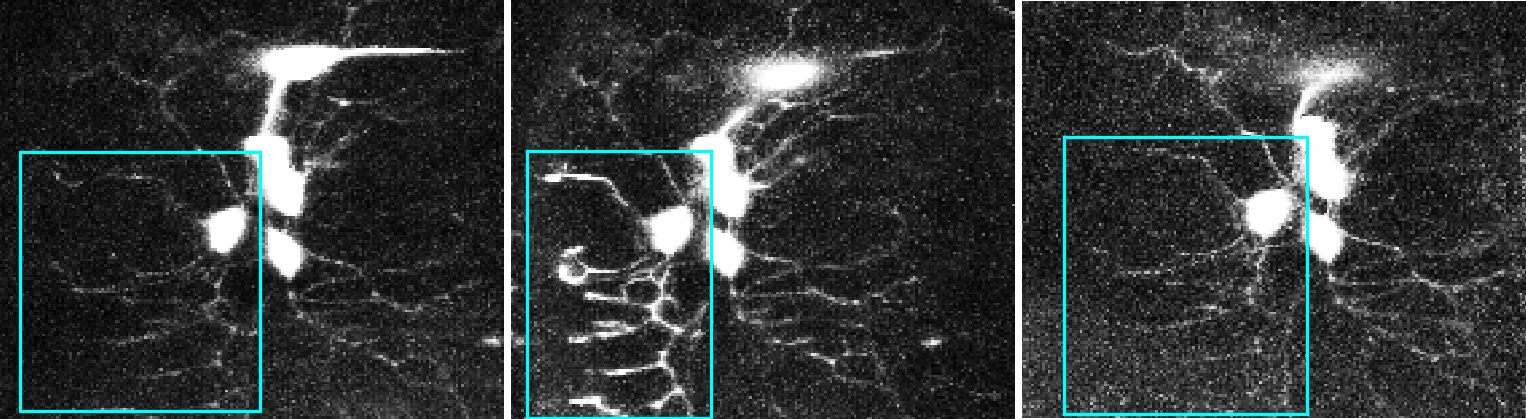
\includegraphics[width=1.0\linewidth]{img/calcium_img}
	\vspace{-20pt}
	\caption{\small{Calcium image characteristics. Three frames of the same neuron (cyan boxes) in temporal order from left to right. First and last frames show inactive neurons so their intensity is low. The middle frame shows the active neuron. Although it has high intensity, it is deforming. Image intensity is adjusted for visualization purposes.}}
	\label{fig:calcium_img}
	\vspace{-10pt}
\end{figure}

% our approach: overview
Here we developed the semi-automatic 3D neuron pose estimation method that can handle these issues and helps reduce the operation time in quantifying both the morphology and neuron activity. It requires little user interaction, including the initial trace and the location of the farthest tips of dendrites, to help handle dendrite detection issues. Then, our method finds the best fits neuron configuration by fitting the neuron plane model surrounding the neuron pair. It incorporates the image feature, neuron local shape, and the domain knowledge about the neuron morphology and deformation during the crawling locomotion. Finally, the deformed traces are efficiently recovered from zthe neuron plane model.


\section{Neuron Plane Model}
% motivation of using neuron plane model
First we present the neuron plane model, which is a simplified representation of the neuron pair. It helps reduce the number of parameters required for describing the deformation of neurons over the image sequences. 

% issue with previous method : neuron tree structure model
% assumption 1: reduce DoF
The main issue of neuron tree structure is that it has high degree of freedom (DoF) and there are insufficient number of constraints to find the acceptable results. To make this problem feasible, first we assume that neuron mass is preserved and it is enclosed by the surface (the layer beneath epidermis). So we can model the deformation of the neuron through the deformation of the enclosing surface.
% assumption 2: reduce number of possible states
Second, we limit the direction of crawling locomotion of samples. Drosophila larvae are observed by putting the samples through a tiny channel to prevent the larvae from moving into another direction except for forward or backward. As a result, we need to model the deformation only in one direction (X-axis).

% definition
With these assumptions, we define the neuron plane model enclosing the neuron pair at time $t$ as the linear chain model of pictorial structures \cite{Felzenszwalb2005} consisting of $2N$ equal-width stripes/parts, ${\bf S}^t = \{s_i^t\}$, for $i = 1,...,2N$ and $t = 0,...,T$ (fig.~\ref{fig:planemodel}). A set of part parameter $\theta^t = \{\theta_i^t\}$ indicating the orientation in XZ-axis of every part at time $t$ (we assume there are no movements in Y-axis). At $t=0$, ${\bf S}^0$ is the bounding box of the initial neuron trace provided by the user, $Y^0$, so it is a flat surface, $\theta_i^0 = 0$, for $\forall i \in [1, 2N]$. $L(s_i^t)$ and $R(s_i^t)$ are the functions indicating the leftmost and rightmost locations of the stripe $s_i^t$ respectively. To standardize the neuron plane model, the middle line of the neuron plane model $R(s_N^t)$, $L(s_{N+1}^t)$ lies between the two soma of a neuron pair. The centroid of soma is detected using the circular Hough transform \cite{Duda1972}.

\begin{figure}[t]
	\centering
	\vspace{-10pt}
	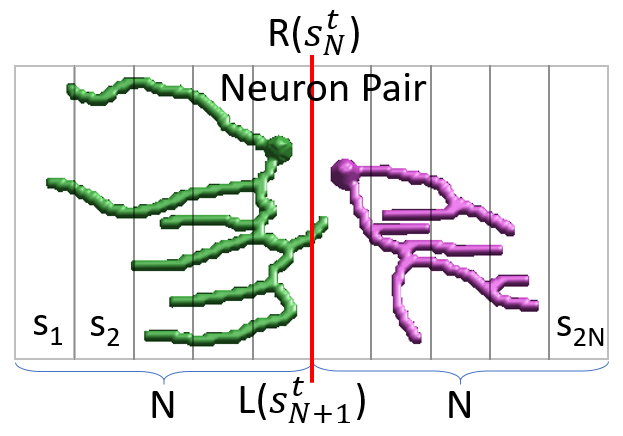
\includegraphics[width=0.5\linewidth]{img/plane_model}
	\vspace{-10pt}
	\caption{\small{Neuron plane model enclosing the neuron pair (green and magenta). The bounding box is split into $2N$ stripes. Its middle line (red line), $L(s_{N+1}^t)$ and $R(s_N^t)$, aligns with the center between soma.}}
	\vspace{-10pt}
	\label{fig:planemodel}
\end{figure}


\section{Optimization}
Calcium image characteristics (fig.~\ref{fig:calcium_img}) makes it challenging to get reliable tracking results in every frame. To tackle this difficulty, our method requires user interaction, including the initial trace, $Y^0$, when the neuron pair is flat and the X-coordinate of the farthest dendrite tips at time $t$, $p^t_k$ (fig.~\ref{fig:ui}). Moreover, we track the neurons indirectly by tracking the neuron-enclosing surface instead using our neuron plane model to improve robustness and efficiency. To convert the initial trace $Y^0$ into the plane model, the number of parts $N$ is picked to be just high enough to enclose the trace and set $\theta_i^0 = 0$.

Given the volume sequence $V = \{V^t\}$, we formulate the objective function as the conditional distribution over the neuron plane parameter, $\theta^t$, at every time step, $\forall t \in [1, T]$:
\begin{equation}
\begin{aligned}
\widehat{\theta}^t & = \argmax_{\theta^t} P(\theta^t | V^t, \theta^{t-1}, p^t_k),  \\
P(\theta^t | V^t, \theta^{t-1}, p^t_k) & \propto \\
& \hspace{-60pt} \exp \Bigg\{ - \sum_{t=1}^T \Big( E_{x}(\theta^t,V^t, p^t_k) + E_{z}(\theta^t,\theta^{t-1}) \Big) \Bigg\}
\end{aligned}
\end{equation}

Although using neuron plane model improves the efficiency in finding the optimal trace configuration $Y^t$ because it has lower number of DoF, we improve its efficiency further by separating the user intervention and automatic steps. So the optimization is divided into two steps --- X-optimization (Sec.~\ref{sec:x-optim}) and Z-optimization (Sec.~\ref{sec:z-optim}), in order to achieve low latency, crucial in interactive approach. Both steps are optimized using the simulated annealing technique \cite{Kirkpatrick1983}.

\begin{figure}[b]
	\centering
	\vspace{-10pt}
	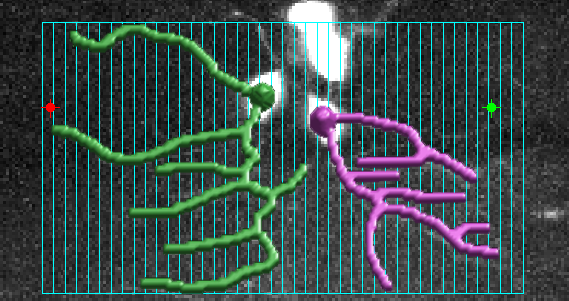
\includegraphics[height=70pt]{img/user_ui}
	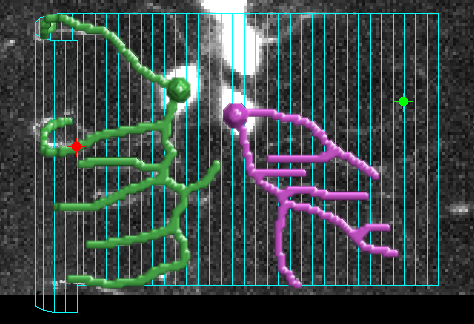
\includegraphics[height=70pt]{img/user_ui13}
	\vspace{-10pt}
	\caption{\small{User interaction required by our method. Red and green points are the X-coordinates of the farthest dendrite tips; and the traces of a neuron pair are in magenta and green color. The neuron plane model is in cyan color. (Left) at $t=0$, the neuron plane model is the loose bounding box of the initial traces $Y^0$. (Right) at $t=12$, the neuron pair is deformed with respect to the deformed neuron plane model.}}
	\vspace{-10pt}
	\label{fig:ui}
\end{figure}


\subsection{X-Optimization} \label{sec:x-optim}
This step finds the neuron plane configuration in X-axis with respect to the user input that best match to the input volumes, while enforcing the constraints of smooth flat surface.
\begin{equation}
\begin{split}
E_{x}(\theta^t,V^t,p^t_k) = & E_{img}(\theta^t,V^t) + E_{shape}(\theta^t) \\
& \quad + E_{flat}(\theta^t) + E_{con}(\theta^t, p^t_k)
\end{split}
\end{equation} 

\textbf{Image feature} term $E_{img}$ selects the neuron plane configuration that maximizes the normalized cross correlation (NCC) \cite{Yoo2009} between the current frame, $V^t$, cropped around the neuron pair and the transformed inital frame, $T(V^0, \theta^t)$, with respect to the neuron plane model (see details of $T$ in Section~\ref{sec:gettrace}). Since the calcium image stacks are noisy, the maximum projection of image stacks, $I^t$, are preferred to make the input images more reliable. 
\begin{equation} \label{eq:Eimg}
E_{img}(\theta^t,V^t) = NCC(I^t, T(I^0, \theta^t))
\end{equation} 

\textbf{Shape energy} term $E_{shape}$ enforces the transformation smoothness over the orientation parameters of the neuron plane model. It is the local shape regularization along X-axis.
\begin{equation}
E_{shape}(\theta^t) = \sum_{i=1}^{2N-1} (\theta_{i+1}^t - \theta_i^t)^2
\end{equation} 

\textbf{Flat surface energy} term $E_{flat}$ encourages flat surface to capture the whole neurons when they start folding. This term helps us decouple the two optimization steps by making this step independent of surface depth.
\begin{equation}
E_{flat}(\theta^t) = \sum_{i=1}^{2N} (\theta_i^t)^2
\end{equation} 

\textbf{Constraint energy} term $E_{con}$ matches the dendrites tips derived from the neuron plane model with the user-given ones. It enforces the constraints provided by users.
\begin{equation} \label{eq:Econ}
E_{con}(\theta^t, p^t_k) = \sum_{k=1}^{2} (p_k^t - T(p_k^0, \theta^t))^2
\end{equation}


\subsection{Z-Optimization} \label{sec:z-optim}
The second step automatically tunes the neuron model configuration in Z-axis according to the input volume and our domain knowledge about the morphology and locomotion. It adjusts the neuron plane model so that it has smooth transition, low curvature, and low depth. Hence, in this step, the value of $\theta_i^t$ is modified by reflecting across the XY-plane. Since it is an automatic step, so it is a part of the post-processing step.
\begin{equation}
E_{z}(\theta^t,\theta^{t-1}) = E_{dep}(\theta^t) + E_{curv}(\theta^t) + E_{tran}(\theta^t,\theta^{t-1})
\end{equation}

\textbf{Depth energy} term $E_{dep}$ adjusts the neuron plane model to have low depth to prevent the model from expanding outside of the input volumes, since image stacks have around 5-10 slices ($\approx ?? \mu m$). %% Ask Liping
\begin{equation}
E_{dep}(\theta^t) = \sum_{i=1}^{2N} \left( D(\theta_i^t) \right)^2
\end{equation} 
where $D(\theta_i^t)$ is the depth of the neuron stripe/part $i$ at time $t$.

\textbf{Curvature energy} term $E_{curv}$ selects low curvature configuration to enforce shape smoothness over XZ-axes and regularize the neuron plane parameters.
\begin{equation}
E_{curv}(\theta^t) = \sum_{i=2}^{2N-1} (R(s_{i+1}^t) - 2L(s_i^t) + L(s_{i-1}^t))^2
\end{equation} 

\textbf{Transition energy} term $E_{tran}$ enforces transition smoothness between consecutive time steps to ensure consistency over sequences.
\begin{equation}
E_{tran}(\theta^t) = \sum_{i=1}^{2N} \left\{ D(\theta_i^{t-1}) - D(\theta_i^t) \right\}^2
\end{equation}


\subsection{Retrieving Deformed Traces} \label{sec:gettrace}
%To recover the deformed neuron traces using the neuron plane model.
The neuron plane model represents the deformation of the initial trace via the uniform cubic B-spline
free-form deformations (FFD) \cite{Rueckert1999}. To recover the deformed neuron traces $Y^t$, first we need to compute the control points ${\bf C}^t = \{c_k^t\}$, which is defined by endpoints of parts.
\begin{equation}
c_k^t = 
\begin{cases}
L(s_{k+1}^t), & \text{if } 0 \leq k \leq N-1 \\
R(s_k^t), & \text{if } N \leq k \leq 2N \\
\end{cases}
\end{equation}

So the transformation from initial time step $t=0$ to the any time step $t$, $T({\bf x}, \theta^t)$, at any point ${\bf x} = (x,y,z)$ is defined as,
\begin{equation}
T({\bf x}, \theta^t) = \sum_{c_k^t \in {\bf C}^t} \eta({\bf x}, c_k^t) {\bf d}_k^t
\end{equation}
where $\eta$ is the coefficient of the control point $c_k^t$ with displacement ${\bf d}_k^t = c_k^t - c_k^0$ at point ${\bf x}$.


\section{Experiments}
% dataset overview
We validated our method on the time-lapse calcium volumes dataset of larval Drosophila sensory neurons. Larvae expressing the genetically encoded calcium sensor GCaMP6.0F in the proprioceptors were observed in four dimensional confocal microscopy imagery. This is achievable because the neurons are found directly beneath the cuticle and epidermis which are optically transparent.

\begin{figure}[b]
	\centering
	\vspace{-10pt}
	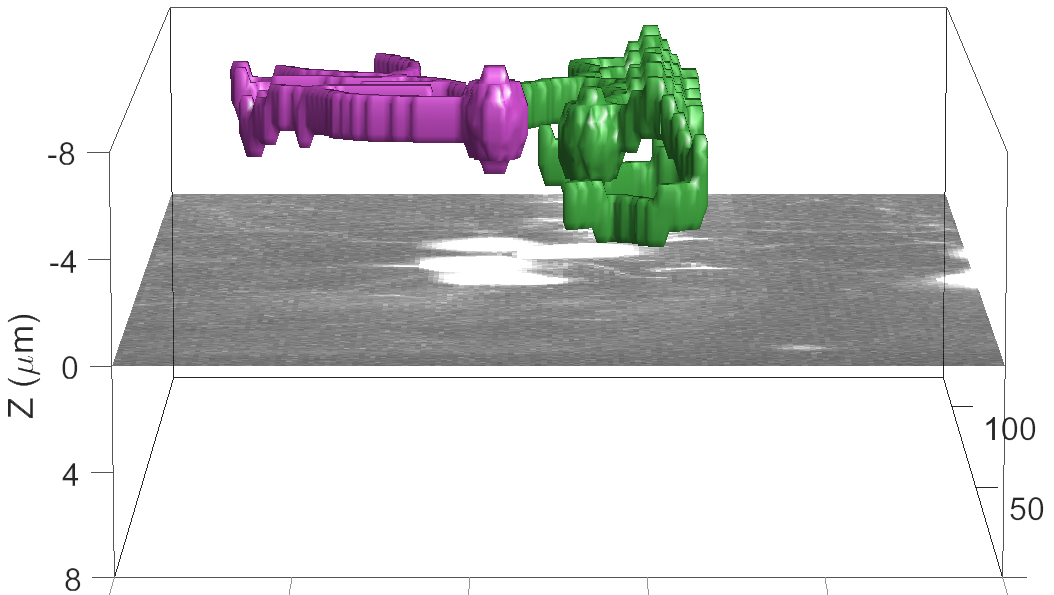
\includegraphics[height=80pt, width=0.45\linewidth]{img/norm2}
	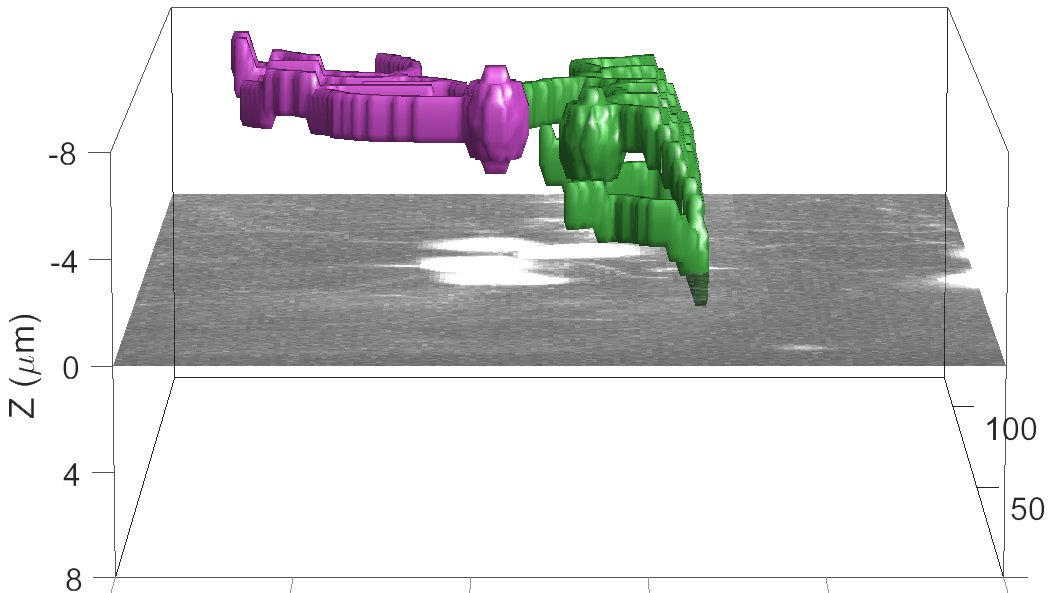
\includegraphics[height=80pt, width=0.45\linewidth]{img/dep2}
	\vspace{-10pt}
	\caption{\small{The importance of depth energy $E_{dep}$ that limits the depth of traces (left) within the image stack (9 slices, $z=0,...,8$ in this example). Otherwise, the depth may be overestimated and higher than the thickness of the image stack (right).}}
	\vspace{-10pt}
	\label{fig:Edep}
\end{figure}

% dataset detail and metric
In this dataset, each sequence captured the neuronal displacement and deformation during the crawling locomotion over 10-50 frames (depends on the movement speed). We measure how well model fits the data using the mutual information (MI) \cite{Viola1997} between artificial volume produced by the deformed initial traces against the input volumes. MI is defined by, $MI(A,B) = \sum_{a \in A}\sum_{b \in B} P(a,b) \log \frac{P(a,b)}{P(a)P(b)}$, where $A$ is the input volume and $B$ is the artificial volume derived from the neuron plane model. Maximizing the mutual information find the best aligned volumes. MI metric is adopted here because it was used in comparing between the model and the volume before \cite{Viola1997}.

%% implementation details
%In our implementation, $\theta_iู^t$ uses the relative orientation instead of the absolute orientation. Then, in X-optimization step, we can limit the possible states of neuron plane parameters, $\theta_i^t \in \{-3\pi/8, -\pi/4, ..., 3\pi/8 \}$.

% significance of each component
Our method is the first for recovering 3D neuron pose from calcium image sequences. Previous works \cite{Ferrari2009, Glowacki2017, Gulyanon2018a} in pose estimations are incapable of handling issues in noisy time-lapse calcium volumes during the locomotion. Table~\ref{tab:result} emphasizes the significance of two novel components, $E_{dep}$ and $E_{flat}$, in our energy function formulation or lack thereof. The depth energy is required to bound the thickness of neurons (fig.~\ref{fig:Edep}). Although the resolution of image stacks in Z-axis is low, the thickness of neurons can still be approximated from the number of image slices and it shows that neurons have low thickness. The flat surface energy encourages the plane to fold rather than squeeze the neurons to match the input volume (fig.~\ref{fig:Eflat}). These two terms help decouple the two optimization steps. 

\begin{figure}[t]
	\centering
	\vspace{-10pt}
	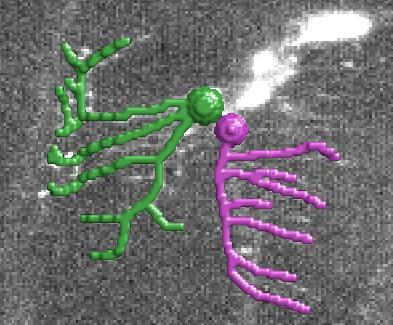
\includegraphics[height=80pt]{img/norm1}
	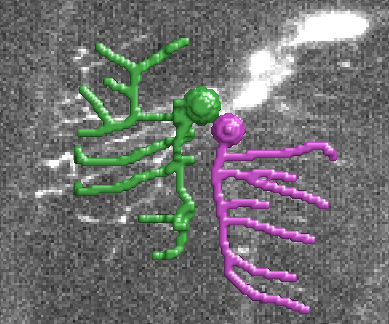
\includegraphics[height=80pt]{img/flat1}
	\vspace{-10pt}
	\caption{\small{The importance of flat surface energy $E_{flat}$. It encourages the neuron plane to fold (left) instead of squeezing it to fit the input volume (right).}}
	\vspace{-10pt}
	\label{fig:Eflat}
\end{figure}


\begin{table}[b]
	\centering
	\vspace{-10pt}
	\begin{tabular}{|c|c|c|c|}
		\hline 
		& Our Method & $E_{dep} = 0$ & $E_{flat} = 0$ \\ 
		\hline 
		Avg & 0.1446 & 0.1380 & 0.1436 \\ \hline
		Std & 0.0342 & 0.0330 & 0.0340 \\
		\hline 
	\end{tabular}
	\vspace{-10pt}
	\caption{\small{The mutual information similarity results between the artificial trace volume produced from the neuron plane model against the input volumes. From left to right: our model, our model without the depth energy term, and our model without the flat surface energy term. The rows show the average and the standard deviation over the volume sequences.}}
	\label{tab:result}
\end{table}


% faster when we separate the optimization
Second, we show the improvement in computation compared to when these two optimization steps are combined. The reason for separating the optimization step is purely for performance. Since this is the semi-automatic method so the performance in term of efficiency is critical for providing quick response time and user interaction. Here, we achieved the average speed around 15 FPS on mid-end computer (Intel Core i7-5500U CPU 2.40 GHz DDR3 8.00GB). If we combines the two steps we end up with just around 3 FPS. The efficiency gain comes from the separation of the automatic process from the user-involved process.


\section{Conclusion}
We presented the semi-automated 3D neuron pose estimation method via neuron plane model for calcium volume sequences. Our method incorporates the image feature, neuron local shape characteristics, and the domain knowledge about the deformation during the crawling locomotion. Our neuron plane model enclosing the neuron pair offers a simplified model. While breaking down the optimization into two steps helps reduces latency to user interactions. Our method is robust to noisy calcium volumes with severe deformations and requires only little user interaction. We validated our results using the time-lapse calcium volumes dataset of larval Drosophila sensory neurons.





%% To start a new column (but not a new page) and help balance the last-page
%% column length use \vfill\pagebreak.
%% -------------------------------------------------------------------------
%\vfill
%\pagebreak


% References should be produced using the bibtex program from suitable
% BiBTeX files (here: strings, refs, manuals). The IEEEbib.bst bibliography
% style file from IEEE produces unsorted bibliography list.
% -------------------------------------------------------------------------
\bibliographystyle{IEEEbib}
%\small{\bibliography{all}}
\small
\begin{thebibliography}{10}
\addtolength{\itemsep}{-1pt}

\bibitem{Hughes2007}
C.~L. Hughes and J.~B. Thomas,
\newblock ``A sensory feedback circuit coordinates muscle activity in
{Drosophila},''
\newblock {\em Mol. Cell. Neurosci.}, vol. 35, no. 2, pp. 383--396, 2007.

\bibitem{Grueber2002}
W.~B. Grueber, L.~Y. Jan, and Y.~N. Jan,
\newblock ``Tiling of the {Drosophila} epidermis by multidendritic sensory neurons,''
\newblock {\em Development}, vol. 129, no. 12, pp. 2867--2878, 2002.

\bibitem{Gulyanon2018a}
S.~Gulyanon, L.~He, W.~D.~Tracey Jr., and G.~Tsechpenakis,
\newblock ``Neurite tracking in time-lapse calcium images using {MRF}-modeled pictorial structures,''
\newblock {\em ISBI}, pp. 1564-1568, 2018.

\bibitem{Ferrari2009}
V.~Ferrari, M.~Marin-Jimenez, and A.~Zisserman,
\newblock ``Pose search: Retrieving people using their pose,''
\newblock {\em CVPR}, pp. 1--8, 2009.

\bibitem{Glowacki2017}
P.~Glowacki, M.~A. Pinheiro, A.~Mosinska, E.~T{\"u}retken, D.~Lebrecht, A.~Holtmaat, R.~Sznitman, J.~Kybic, and P.~Fua,
\newblock ``Reconstructing evolving tree structures in time lapse sequences by enforcing time-consistency,''
\newblock {\em TPAMI}, vol. PP, no. 99, pp. 1--1, 2017.

\bibitem{Gulyanon2017}
S.~Gulyanon, N.~Sharifai, M.~D. Kim, A.~Chiba, and G.~Tsechpenakis,
\newblock ``Neurite reconstruction from time-lapse sequences using co-segmentation,''
\newblock {\em ISBI}, pp. 410--414, 2017.

\bibitem{Felzenszwalb2005}
P.~F. Felzenszwalb and D.~P. Huttenlocher,
\newblock ``Pictorial structures for object recognition,''
\newblock {\em IJCV}, vol. 61, no. 1, pp. 55--79, 2005.

\bibitem{Duda1972}
R.~O. Duda and P.~E. Hart,
\newblock ``Use of the hough transformation to detect lines and curves in pictures,''
\newblock {\em Commun. ACM}, vol. 15, no. 1, pp. 11--15, 1972.

\bibitem{Kirkpatrick1983}
S.~Kirkpatrick, C.~D. Gelatt, and M.~P. Vecchi,
\newblock ``Optimization by simulated annealing,''
\newblock {\em Science}, vol. 220, no. 4598, pp. 671--680, 1983.

\bibitem{Yoo2009}
J.-C. Yoo and T.~H. Han,
\newblock ``Fast normalized cross-correlation,''
\newblock {\em Circuits, Systems and Signal Processing}, vol. 28, no. 6, pp. 819, 2009.

\bibitem{Rueckert1999}
D.~Rueckert, L.~I. Sonoda, C.~Hayes, D.~L.~G. Hill, M.~O. Leach, and D.~J.
Hawkes,
\newblock ``Nonrigid registration using free-form deformations: Application to breast {MR} images,''
\newblock {\em IEEE Trans. Med. Imag.}, vol. 18, no. 8, pp. 712--721, 1999.

\bibitem{Viola1997}
P.~Viola and W.~M.~Wells III,
\newblock ``Alignment by maximization of mutual information,''
\newblock {\em IJCV}, vol. 24, no. 2, pp. 137--154, 1997.
\end{thebibliography}


\end{document}
